% Tento soubor nahraďte vlastním souborem s obsahem práce.
%=========================================================================
% Autoři: Michal Bidlo, Bohuslav Křena, Jaroslav Dytrych, Petr Veigend a Adam Herout 2019
\chapter{Úvod}
\label{uvod}

Na pozadí počítačovej hry sa odohráva veľký počet komplexných činností, ktoré častokrát uživateľ, respektíve hráč, nevidí. V závodnej hre by medzi tieto činnosti patrilo napríklad výpočet fyziky áut, prehrávanie zvuku motora vzhľadom od aktuálnej rýchlosti alebo zaradeného stupňa, prehrávanie zvuku okolitého prostredia, aktualizácia dát v uživateľskom rozhraní a interakcia s ním. Zariadenie na ktorom táto hra beží ma ale obmedzený výpočetný výkon, ktorý je potrebné medzi tieto činnosti rozložiť. Činnosť ktorá trvá príliš dlho, ovplyvňuje tie ostatné a prejaviť sa to môže napríklad formou oneskorenia a zasekávania. Za takúto činnosť je možné považovať napríklad vykresľovanie, ktoré vyžaduje značnú časť výpočetného výkonu. Navyše značne narastá pri vysokom počte a zložitosti prvkov, ktoré je potrebné vykresliť. Tento problém začal byť naprieč 90. rokmi natoľko limitujúci, že bolo potrebné presunúť tieto výpočty z CPU na inú komponentu zariadenia, ktorá by ich počítala rýchlejšie a efektívnejšie.

Základ počítačov, CPU, má poskytovať flexibilnú a všestrannú funkcionalitu pre implementáciu akéhokoľvek algoritmu. Výpočetný výkon CPU je ale na niektoré algoritmy a činnosti príliš pomalý. Grafické karty, ďalej len GPU, boli originálne vytvorené za účelom zrýchlenia vykresľovania 3D objektov a práce s textúrami. Ich paralelná štruktúra zaručuje vysokú efektivitu špecifických algoritmov, oproti CPU niekoľkonásobne, ktoré potrebujú pracovať paralelne s veľkým objemom dát. Naprieč rokmi sa GPU stali flexibilnejšími, využívajú sa v rôznych technologických sektoroch a ich použitie už nieje cielené iba na hry.

CPU sa dá predstaviť ako švajčiarsky nôž a GPU ako mačeta. Švajčiarsky nôž je nápomocný pri množstve rôznych úloh, od prestrihnutia lana až po otvorenie plechovky s fazuľou. Keď sa však chceme predierať hustou džungľou, využijeme silnú mačetu, nie malý švajčiarsky nôž.

\section{Ciele práce}

Hlavným cieľom tejto práce je vytvoriť nástroj pre tvorbu hier takých, že celá vrátane vykresľovania a vnútornej logiky pobeží na GPU. Práca má taktiež za úlohu nájsť limity a prednosti tohto spôsobu tvorby hier a porovnať ho z klasickým spôsobom, kde sa stále prevažne využíva CPU na väčšinu výpočtov logiky hry.

\chapter{Teória}

Táto časť popisuje všetký podstatné informácie pre tému tejto práce, teda popis GPU, porovnanie GPU s CPU, spôsob práce s GPU a dostupné nástroje pre tvorbu hier.

\section{GPU}

GPU má radu využití, obzvlášť vykresľovanie, ale aj napríklad strojové učenie alebo ťaženie kryptomien. Ak vynecháme použitia GPU, ktoré sa rozšírili hlavne poslednými rokmi a v tejto práci nie sú podstatné, môžeme GPU definovať ako "Výpočetnú jednotku zariadenia pre akceleráciu komplexných matematických a geometrických výpočtov, ktoré sú nutné pre grafické vykresľovanie.". 

\subsection{Jadro}
GPU podobne ako aj CPU sa skladá z jadier. 

\begin{itemize}
  \item{\bf Jadro \rm je samostatná výpočetná jednotka, ktorá prijíma inštrukcie pracujúce s nejakými dátami a vykonáva výpočty alebo operácie pre uspokojenie týchto inštrukcií.}
\end{itemize}

\subsection*{Jadro CPU}
CPU jadro je schopné širokého spektra operácií a vysporiadava sa s tokom inštrukcií. Viaceré programy súperia o výpočetný čas, ktorý im je prideľovaný operačným systémom. Inštrukcie pracujú s dátami uloženými v pamäti RAM. Tento prenos je relatívne pomalý nakoľko pamäť RAM nieje súčasťou CPU. Z toho dôvodu si CPU uchováva niektoré dáta vo vyrovnávacej pamäti, takzvanej CPU cache, za účelom minimalizácie prístupu k pamäti RAM.

Spracovanie veľkého počtu inštrukcií benefituje z vysokej rýchlosti jednotlivého jadra, pretože môže byť obtiažne rozdeliť jeden tok inštrukcií na niekoľko menších. Pre toto spracovanie je teda vhodnejší menší počet výkoných jadier.

\subsection*{Jadro GPU}
GPU jadro je na druhej strane navrhnuté pre prácu s datovými tokmi. Jednotlivé jadra pracujú s minimálnym počtom inštrukcií, ktoré pracujú s potencionálne veľkým počtom dát. Grafické karty majú vlastnú pamäť, zvanú video pamäť, v ktorej si dáta s ktorými pracujú ukladajú. Vzhľadom na to, že táto pamäť je súčasťou grafickej karty, je rýchlosť prenosu medzi ňou a jadrami niekoľkonásobne vyššia ako v prípade CPU komunikujúcim s pamäťou RAM. Samotné jadrá v moderných GPU zdieľajú tok inštrukcií za účelom minimalizácie réžie jednotlivých jadier.

\label{gpulogic}
Spracovanie veľkého množstva dát častokrát znamená vykonávanie rovnakej činnosti nad rôznymi dátami, častokrát definovanej malým počtom inštrukcií. Pre takéto spracovanie je teda výhodný paralelizmus a vysoký počet jadier. Pre príklad môžeme uviesť vykresľovanie objektov, kde sa vykonáva ten istý algoritmus nad potencionálne obrovským počtom objektov.

\subsection*{Časti jadra}
V čom spočíva efektivita GPU jadier oproti CPU jadrám? Na to aby bolo možné túto otázku zodpovedať, je potrebné začať rozložením častí CPU jadra.

\begin{figure}[H]
	\centering
	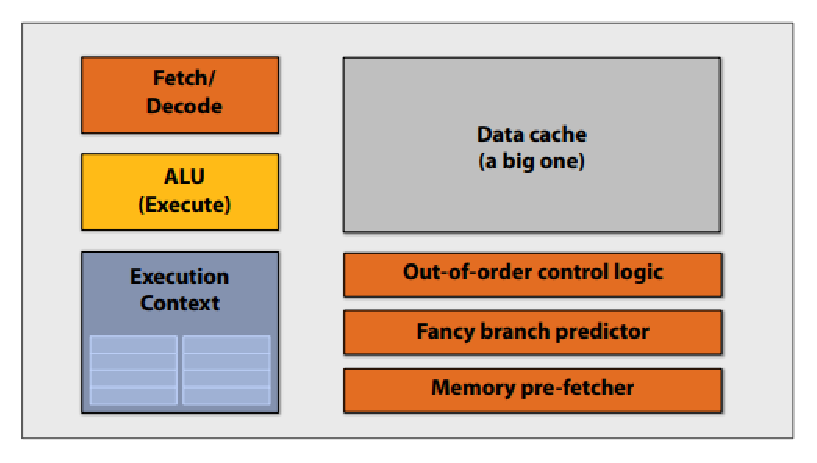
\includegraphics[width=0.7\textwidth]{obrazky-figures/cpucore.eps}
	\caption{Rozloženie častí CPU jadra.}
	\label{cpucore}
\end{figure}

Jadro CPU funguje na princípe fetch/decode/execute. Teda načíta inštrukciu - fetch, dekóduje ju - decode a následne vykoná - execute. Stav procesoru, teda obsahy registrov a programový čítač je uložený v execution kontexte. Data cache obsahuje lineárne časti pamäte RAM, ktoré si CPU dočasne uchováva pomocou prefetcheru za účelom minimalizácie k jej prístupu, keďže ako už bolo spomenuté, je to relatívne pomalé a CPU potrebuje inštrukcie odbavovať čo najrýchlejšie. Pre zvýšenie efektivity CPU taktiež využíva predikciu vetvenia, kde sa snaží CPU uhádnuť smer vetvy, predtým ako je to definitívne známe. Posledná časť je vykonávanie inštrukcií v inom ako ich definovanom poradí. Pokiaľ procesor čaká na dokončenie nejakej inštrukcie, je možné medzitým vykonať následujúce inštrukcie, ktoré na nej nezávisia. To závisí od dát a jednotiek s ktorými inštrukcia pracuje.

Funkcionalita ktorú obsahujú CPU jadrá prináša so sebou navýšenie réžie. Keďže GPU dnes dosahujú tisíce jadier, je táto réžia neprípustná. Ako už bolo povedané v popise GPU jadra, viz. \ref{gpulogic}, je účelom jadier paralelne vykonávať rovnakú činnosť. Nieje teda nutné aby každé GPU jadro obsahovalo podobné časti a funkcionalitu ako CPU jadro.

\begin{figure}[H]
	\centering
	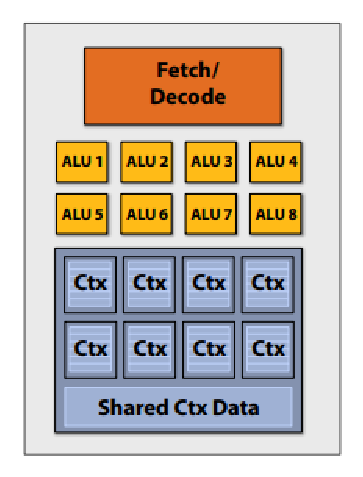
\includegraphics[width=0.3\textwidth]{obrazky-figures/gpucore.eps}
	\caption{Rozloženie častí GPU jadra.}
	\label{gpucore}
\end{figure}

Jadro GPU funguje taktiež na princípe fetch/decode/execute. Jedným z rozdielov medzi GPU a CPU je ten, že GPU dostane úlohu, respektíve program, a čaká sa na jej výsledok. Programov na CPU beží veľa naraz, niektoré nikdy nekončia, niektoré vykonávajú akcie počas ktorých môžu byť odložené a spustené neskôr. GPU jadro vďaka tomu nepotrebuje tak pokročilé mechanizmy na zefektívnenie toku inštrukcií. Samotné GPU jadro teda načíta inštrukciu ktorú má vykonať. Obsahuje viacero aritmetických logických jednotiek - ALU a bloky kontextov, ktoré tieto ALU využívajú. Tento princíp sa nazýva SIMD - Single Instruction Multiple Data. Kontexty majú vlastné dáta ale aj zdieľané medzi sebou.

\label{pixelex}
\begin{itemize}
  \item{Príklad využita viacerých kontextov a výpočetných jednotiek môže byť napríklad výpočet 8 pixelov na obrazovke. Jadro si načíta inštrukciu pre výpočet farby pixelu. Každý z týchto 8 pixelov má vlastný context, ktorý obsahuje napríklad jeho pozíciu. Jednotlivé kontexty jadro spracuje paralelne pomocou dostupných ALU jednotiek. Počet jednotiek ALU a kontextov v jednotlivých jadrách závisí od samotnej GPU.}
\end{itemize}

\begin{figure}[H]
	\centering
	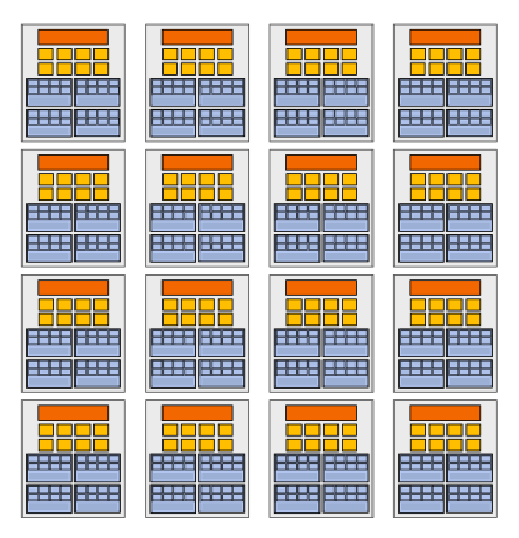
\includegraphics[width=0.5\textwidth]{obrazky-figures/gpucores.eps}
	\caption{Viacero jadier GPU.}
	\label{gpucores}
\end{figure}

Na obrázku \ref{gpucores} je možné vidiet predstavu viacero GPU jadier, kde môžeme vidieť 16 jadier. Každé jadro obsahuje 4 bloky kontextov, kde každý blok obsahuje 8 kontextov. V prípade aplikácie príkladu o pixeloch \ref{pixelex} na tento obrázok, by sme mohli paralelene vypočítať farbu 512 pixelov.

\begin{equation}
	16 * 4 * 8 = 512
	\label{eq:pixeleq}
\end{equation}

\subsection*{Logická organizácia práce}
\label{workgrouplogic}
Pri práci s GPU nepracujeme priamo s jadrami. Využíva sa pojem globálnych a lokálnych pracovných skupín, do ktorých je rozdelená požadovaná práca vo forme pracovných jednotiek. Pracovná jednotka je najmenšia jednotka zapúzdrujúca operácie, ktorú môže uživateľ vykonať.
Pracovné skupiny sú definované v 3D priestore. Akákoľvek z osí priestoru môže byť 1, čo je vhodné pre spracovanie akýchkoľvek obrazových dát alebo lineárnych dát. Pracovné skupiny sú vykonávané paralelne, nezávisle od iných.

\begin{figure}[H]
	\centering
	\includegraphics[width=0.6\textwidth]{obrazky-figures/workgroups.eps}
	\caption{Organizácia pracovných skupín.}
	\label{workgroups}
\end{figure}

\begin{itemize}
  \item{\bf Globálna skupina \rm je pracovná skupina, ktorej jednotky predstavujú lokálne skupiny. Globálne skupiny sú vykonávané nezávisle na sebe.}
  \item{\bf Lokálna skupina \rm je pracovná skupina, ktorej jednotky predstavujú spustenie programu, ktoré využívajú svoju pozíciu v priestore a častokrát pracujú s jemne odlišnými dátami. Lokálne skupiny sú vykonávané nezávisle na sebe, ale samotné jednotky lokálnej skupiny je možné medzi sebou synchronizovať.}
\end{itemize}

V prípade vykonania pracovných skupín na základe obrázku \ref{workgroups}, teda globálna skupina veľkosti (X=2, Y=3, Z=3) a lokálna skupina veľkosti (X=7, Y=5, Z=3), by sme dostali 1890 jednotlivých spustení programu, kde v každom spustení môžeme pracovať s inými dátami.

\begin{equation}
	(2*3*3) * (7*5*3) = 1890
	\label{eq:workgroupeq}
\end{equation}

Veľkosť pracovných skupín sa prispôsobuje požiadavkam programu, ktorý bude spúšťaný na GPU. Je možné spraviť aj 1 globálnu skupinu (X=1, Y=1, Z=1) s 1 lokálnou skupinou (X=1, Y=1, Z=1), ktorá by vykonala program iba raz.

\subsection*{Kedy použiť GPU a kedy CPU}
Na teoretickej úrovni je častokrát možné dosiahnuť toho istého cieľa na CPU aj GPU, no spôsob jeho dosiahnutia by sa líšil vzhľadom na ich odlišný princíp. Na základe spôsobu akým fungujú, je GPU ideálne pre všeobecne zamerané toky inštrukcií, a GPU je ideálne pre prácu s veľkým objemom dát. 

\subsection{Program}

\begin{itemize}
  \item{\bf Program \rm je sekvencia alebo zoznam inštrukcií v nejakom programovacom jazyku, ktoré môže počítač interpretovať alebo vykonať.}
\end{itemize}

Programy na CPU sú definované inštrukciami, ktoré samotné CPU podporuje a ich forma sa naprieč rokmi podstatne nemení. Tieto inštrukcie sú zapísané v takzvanom assembly code, ktorý je určený pre priamu komunikáciu s hardwarom. Rôzne kompilované programovacie jazyky sú kompilované do assembly code, ktorý je následne skompilovaný do strojového kódu spustiteľného na CPU na danom operačnom systéme.

Programy na GPU sú taktiež definované inštrukciami, ale forma týchto inštrukcií a spôsob ich použitia sa častokrát mení v každej GPU pre zaručenie najvyššej efektivity. Z toho dôvodu nieje väčšinou inštrukčná sada GPU verejne dostupná a komunikácia prebieha inak. GPU potrebuje ovládač, ktorý implementuje rôzne verejne popísané API, pomocou ktorých je možné s GPU pracovať. Následne je možné v programoch bežiacich na CPU volať funkcie popísané týmito API. Jednou z funkcií týchto API je nahranie programu, respektíve jeho zdrojového kódu na GPU, kde je následne skompilovaný do optimalizovaného strojového kódu, ktorý je možné na GPU spustiť. 

Programy GPU si typicky vopred definujú prostriedky s ktorými chcú na GPU pracovať a ako sa majú na GPU logicky rozložiť \ref{workgrouplogic}

\subsection{API}

\begin{itemize}
  \item{\bf Application Programming Interface - API \rm je zoznam funkcií alebo procedúr umožňujúcich vytváranie aplikácií, ktoré pristupujú k funkciám alebo dátam operačného systému, aplikácie alebo inej služby.}
\end{itemize}

Komunikácia s GPU prebieha prostredníctvom programu spúšťaného na CPU, ktorý volá funkcie popísané API implementovanou ovládačom GPU. Takýchto API existuje v dnešnej dobe viac a každá má svoje vlastné využitie. Medzi najznámejšie a najviac používané patrí

\begin{itemize}
  \item{\bf OpenCL \rm - API pre tvorbu programov všeobecného účelu, spustiteľných na viacerých zariadeniach ako napríklad CPU, GPU alebo FPGA.}
  \item{\bf CUDA \rm - API podobne ako OpenCL využívaná pre tvorbu programov všeobecného účelu, spustiteľných na GPU. Je to proprietárna technológia pre GPU vyrobené firmou NVIDIA.}
  \item{\bf OpenGL \rm - API využívaná najmä pre vykresľovanie 3D grafiky. Je podporovaná takmer všetkými modernými GPU a niektoré jej implementácie majú verejne dostupný zdrojový kód. Jej prvotné verzie boli pomerne obmedzené a poskytovali obmedzenú funkcionalitu schovanú za pomerne vysokou abstrakciou. Naprieč rokmi bola táto funkcionalita rozdelená za účelom zníženia abstrakcie a teda poskytnutia vyššej flexibility vývojárom. Programy popisuje vlastným programovacím jazykom GLSL, ktorého syntax je založená na jazyku C.}
  \item{\bf Vulkan \rm - API novej generácie, ktorá by mala nahradiť OpenGL. Obsahuje minimum abstrakcií oproti OpenGL a teda jej réžia je minimálna. Programy popisuje formátom SPIR-V, ktorý môže pripomínať obdobu assembly kódu pri CPU. Je teda možné využiť viaceré programovacie jazyky, ktoré sú následne skompilované do SPIR-V, teda aj GLSL.}
  \item{\bf DirectX \rm - API využívaná podobne ako OpenGL a Vulkan pre vykresľovanie 3D grafiky. Táto API je proprietárna pre systém Windows a hernú konzolu Xbox a jej implemntácia nieje verejne dostupná. Zariadenia so systémom Windows podporujú aj ostatné populárne API. Jej staršie verzie fungovali na podobnom princípe ako OpenGL, kdežto najnovšia verzia tejto API, DirectX 12, funguje na podobnom princípe ako Vulkan. Programy popisuje programovacím jazykom HLSL, ktorého syntax je, podobne ako ostatné API, založená na jazyku C.}
  \item{\bf Metal \rm - Proprietárna API pre zariadenia Apple pre prácu s GPU. Najnovšie zariadenia Apple nepodporujú Vulkan a novšie verzie OpenGL, a teda vývojárovi na tejto platforme nedáva inú možnosť ako pracovať s touto API. Existujú nástroje ktoré tento problém riešia, napríklad MoltenVK, ktorého úlohou je preklad volania funkcionality API vulkan na ekvivalentné volania API Metal.}
\end{itemize}

Vzhľadom na to že táto práca je zameraná primárne na grafické vykresľovanie, je pozornosť venovaná primárne API OpenGL, kvôli relatívne jednoduchému a jasnému použitiu.

\section{OpenGL}

OpenGL je voľne dostupná a multi platformová API pre prácu s 2D a 3D grafikou, vyvinutá organizáciou Khronos. Je definovaná ako zoznam funkcií a konštánt, ktoré môže klientsky program bežiaci na CPU využiť, respektíve zavolať. Ponúka viaceré abstrakcie pre uľahčenie práce s GPU a grafikou všeobecne.

\subsection*{Shader}

V OpenGL sa spúšťaný program skladá z viacerých menších programov zvaných shader. Tento shader je na GPU nahraný v textovej podobe, v jazyku GLSL. Tá je následne skompilovaná do formy ktorú je GPU schopné spustiť. Existuje viacero typov shaderov, kde každý shader má vlastný účel a vopred definované vstupy a výstupy. Shadre v programe majú určené poradie a sú súčasťou grafickej pipeline, ktorá definuje poradie jednotlivých častí vykresľovania.

\begin{figure}[H]
	\centering
	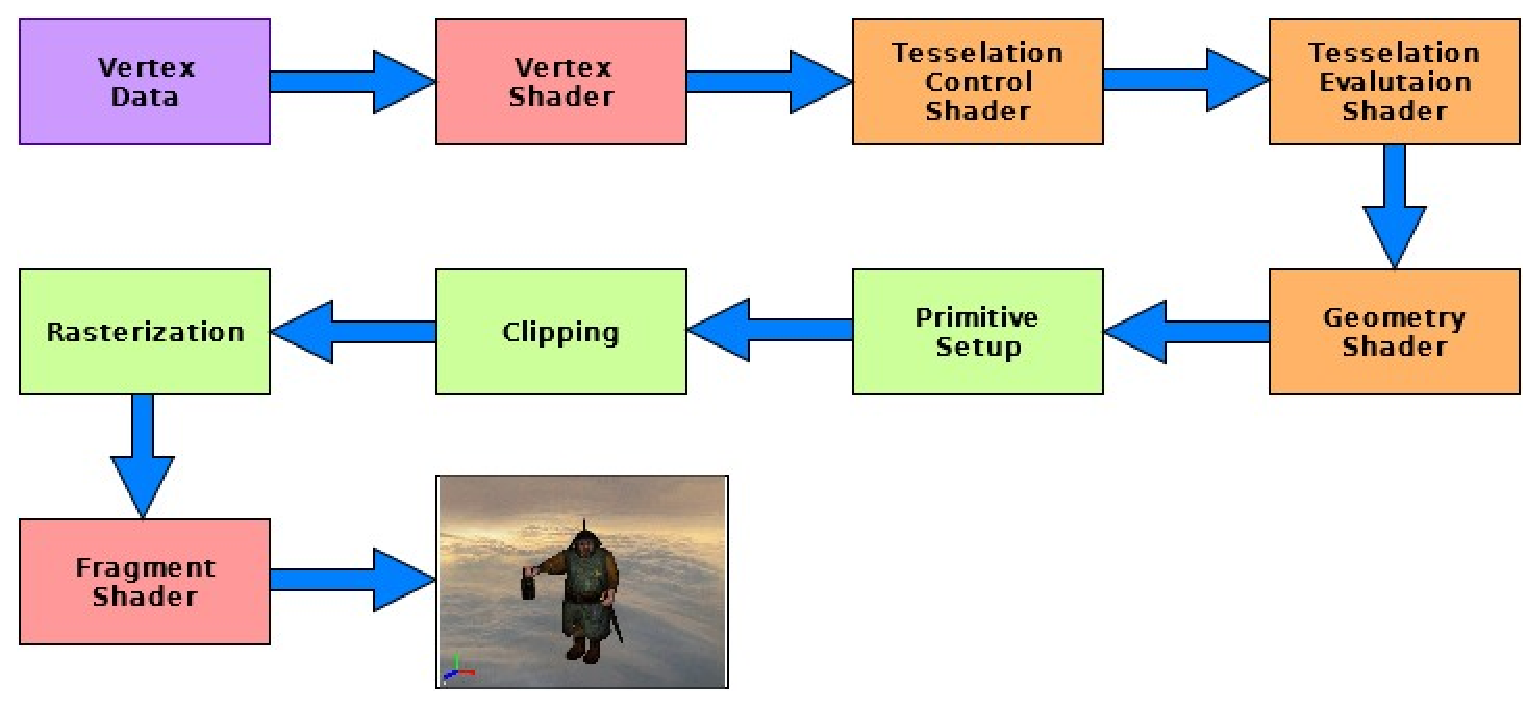
\includegraphics[width=0.8\textwidth]{obrazky-figures/pipeline.eps}
	\caption{Grafická pipeline.}
	\label{pipeline}
\end{figure}

\begin{itemize}
    \item{\bf Vertex data \rm predstavuje vstup grafickej pipeline. Je to zoznam vrcholov primitívnych objektov, typicky trojuholníkov.}
    \item{\bf Vertex Shader \rm je prvý shader grafickej pipeline, ktorý má za úlohu spracovať vrcholy primitívneho objektu. V tomto shaderi je napríklad možné upraviť pozície vrcholov tak, aby odpovedali pozícii kamery scény.}
    \item{\bf Tesselation Shader \rm je shader, pomocou ktorého je možné rozdeliť primitívny objekt na niekoľko menších, za účelom manipulácie s detailom objektu. Vďaka tomuto shaderu je možné napríklad z kocky, ktorá je definovaná 8 vrcholmi, spraviť hladkú guľu, ktorá by musela mať oveľa viac vrcholov.}
    \item{\bf Geometry Shader \rm je shader, ktorý má na vstupe zoznam vrcholov ktoré formujú primitívny objekt, napríklad bod alebo trojuholník. Tie môže následne ľubovoľne transformovať a poslať ďalej. Shader teda môže prijať napríklad jeden bod, a vytvoriť z neho trojuholník so stredom v tomto bode.}
    \item{\bf Clipping \rm je interná záležitosť grafickej karty, ktorá na základe nejakých podmienok zahodí primitívne objekty. Typicky sa jedná o objekty ktoré sa nachádzajú mimo obrazovky a teda ich nieje potrebné vykresľovať.}
    \item{\bf Rasterizácia \rm je predposledná časť pipeline. Prevádza primitívne objekty definované vrcholmi na rastrový obrázok, teda sériu pixelov, zvaných fragmenty.}
    \item{\bf Fragment Shader \rm je shader, ktorý má na vstupe fragmenty vytvorené v rasterizácii. Je možné s nimi manipulovať, napríklad zmeniť ich farbu. Výstupom fragment shaderu je výsledný obraz.}
\end{itemize}

Program v OpenGL ktorý má za úlohu vykresliť obraz môže byť teda definovaný 4 shadermi. OpenGL má ale ešte jeden dôležitý typ shaderu, ktorý je podstatný pre prácu s niečim iným ako vykresľovaním. Jedná sa o Compute Shader, ktorý sa používa na výpočet ľubovoľných informácií. Computer shader môže aj vykresľovať, ale vo väčšine prípadov sa používa pre úlohy, ktoré s vykresľovaním priamo nesúvisia. Compute shader nieje možné kombinovať s inými typmi shadrov vrámci jedného programu.

\subsection*{Textúra}
Textúra je typicky 2D obraz, pomocou ktorého nanášame na časti objektu detaily. Pomocou OpenGL je možné textúru manuálne vytvoriť a nahrať do nej dáta. V jednotlivých shaderoch je následne možné s textúrami pracovať.

\subsection*{Buffer}
Buffer je vyhradená časť video pamäte GPU s prideleným identifikátorom, pomocou ktorého môžeme s týmto blokom pamäte pracovať. Dáta uložené v bufferoch je možné modifikovať, čítať a meniť ich veľkosť. Buffery je možné naviazať na konkrétny typ. Jednotlivé shadre a interné funkcie OpenGL očakávajú dáta v konkrétnych typoch bufferov. 

\subsection*{Framebuffer}
Fragment shader sám o sebe nevykresľuje svoj výstup priamo na obrazovku. Výstup je uložený do bloku pamäte, zvaného framebuffer. V OpenGL existuje predvolený framebuffer, do ktorého sa ukladá výstup určený pre obrazovku. Je možné vytvoriť dodatočné framebuffery, ktoré sa mapujú na textúry, s ktorými ďalej možeme pracovať.

\subsection*{Uniformná premenná}
Uniformná premenná je globálna premenná shaderu. Predstavuje parameter, ktorý môže uživateľ shaderu odoslať. Shader môže tento parameter využiť ľubovoľne podľa potreby.

\subsection*{SSBO}
SSBO, alebo Shader Storage Buffer Object, je taktiež premenná shaderu, ktorá sa chová podobne ako uniformná premenná. Rozdiel spočíva v tom, že veľkosť SSBO môže byť oveľa vyššia a je možné do nich zo shaderu zapisovať, nie len z nich čítať. Je možné teda napríklad využiť program s Compute Shaderom, ktorý svoj výpočet uloží do SSBO a výsledky sa následne použijú v inom programe.

\section{Dostupné nástroje pre tvorbu hier}